\newpage
\section{Phương trình, bất phương trình mũ và lôgarit}
\subsection{LÝ THUYẾT CẦN NHỚ}
\subsubsection{Tính đơn điệu của hàm số}
\indam{Định nghĩa:}
\begin{dn}
	Phương trình dạng $a^x=b$, trong đó $a$ và $b$ là những số cho trước, $a>0$, $a\neq 1$, được gọi là \textbf{\textit{phương trình mũ cơ bản}}.
\end{dn}
\textbf{\color{red} Nghiệm của phương trình mũ cơ bản}: Cho phương trình $a^x=b$ $(a>0, a\neq 1)$
\begin{itemize}
	\item Nếu $b>0$ thì phương trình luôn có nghiệm duy nhất $x=\log_a b$.
	\item Nếu $b\leqslant 0$ thì phương trình vô nghiệm.
\end{itemize}
\begin{note}
	\begin{itemize}
		\item Nếu $b=a^\alpha $ thì ta có $a^x=a^\alpha \Leftrightarrow x=\alpha$.
		\item Tổng quát hơn, $a^{u(x)}=a^{v(x)}\Leftrightarrow u(x)=v(x)$.
	\end{itemize}
\end{note}


\subsubsection{Phương trình lôgarit}
\begin{dn}
	Phương trình dạng $\log _a x=b$, trong đó $a$, $b$ là những số cho trước, $a>0$, $a \neq 1$, được gọi là \textbf{ phương trình lôgarit cơ bản}.
\end{dn}
\textbf{\color{red} Nghiệm của phương trình lôgarit cơ bản}: Phương trình $\log _a x=b$ ($a>0$, $a \neq 1$) luôn có nghiệm duy nhất $x=a^b$.
\begin{note}
	Tổng quát, xét phương trình dạng
	$$\log _a u(x)=\log _a v(x) \quad(a>0, a \neq 1) \quad \quad (1)$$
	Để giải phương trình (1), trước hết cần đặt điều kiện có nghĩa: $u(x)>0$ và $v(x)>0$.\\
	Khi đó, (1) được biến đổi thành phương trình
	$$u(x)=v(x).\quad \quad (2)$$
	Sau khi giải phương trình (2), ta cần kiểm tra sự thoả mãn điều kiện. Nghiệm của phương trình (1) là những nghiệm của (2) thoả mãn điều kiện.
\end{note}
\subsubsection{Bất phương trình mũ}
\begin{dn}
	\textbf{\textit{Bất phuơng trình mũ cơ bản}} là bất phương trình có dạng $a^x>b$ (hoặc $a^x \geq b$, $a^x<b$, $a^x \leq b$), với $a$, $b$ là những số cho trước, $a>0$, $a \neq 1$.
\end{dn}
\textbf{\color{red} Nghiệm của bất phương trình mũ $a^x>b$}\\
\begin{itemize}
	\item Nếu $b \leq 0$ thì mọi $x \in \mathbb{R}$ đều là nghiệm của bất phương trình.
	\item Nếu $b>0$ thì:
	\begin{itemize}
		\item Với $a>1$, nghiệm của bất phương trình là $x>\log _a b$;
		\item Với $0<a<1$, nghiệm của bất phương trình là $x<\log _a b$.
	\end{itemize}
\end{itemize}
\begin{note}
	\begin{itemize}
		\item Tương tự như trên, ta nhận được kết quả về nghiệm của mỗi bất phương trình $a^x \geq b$, $a^x<b$, $a^x \leq b$ (các bất phương trình $a^x<b$, $a^x \leq b$ vô nghiệm nếu $b \leq 0$).
		\item Nếu $a>1$ thì $a^{u(x)}>a^{v(x)} \Leftrightarrow u(x)>v(x)$.\\
		Nếu $0<a<1$ thì $a^{u(x)}>a^{v(x)} \Leftrightarrow u(x)<v(x)$.
	\end{itemize}
\end{note}
\subsubsection{Bất phương trình lôgarit}
\begin{dn}
	\textbf{\textit{Bất phương trình lôgarit cơ bản}} là bất phương trình có dạng $\log _a x>b$ (hoặc $\log _a x \geqslant  b$, $\log _a x<b$, $\log _a x \leqslant  b$), với $a$, $b$ là những số cho trước, $a>0$, $a \neq 1$.
\end{dn}
\textbf{\color{red} Giải bất phương trình $\log_a x>b$ (*)}
\begin{itemize}
	\item Với $a>1$, nghiệm của (*) là $x>a^b$.
	\item Với $0<a<1$, nghiệm của (*) là $0<x<a^b$.
\end{itemize}
\begin{note}
	\begin{itemize}
		\item Nếu $a>1$ thì $\log _a u(x)>\log _a v(x) \Leftrightarrow u(x)>v(x)>0$.
		\item Nếu $0<a<1$ thì $\log _a u(x)>\log _a v(x) \Leftrightarrow 0<u(x)<v(x)$.
	\end{itemize}
\end{note}

%-----------------------------------------------------------------------------
\subsection{Phân loại và phương pháp giải toán}

\begin{dang}{Phương trình mũ, lôgarit cơ bản} 
	Sử dụng các công thức
	\begin{itemize}
		\item $a^{f(x)}=b \Leftrightarrow f(x)=\log_a b$ ($a,b>0$; $a\neq 1$).
		\item $\log_a f(x)=b\Leftrightarrow f(x)=a^b$ ($a>0$; b$a\neq 1$).
	\end{itemize}
\end{dang}

\begin{vd}%[1D6H4-1]%[Dự án đề cương 3 Khối NH 24-25- Dot 1- Nguyễn Trần Anh Tuấn]
	Tìm tất cả các giá trị $m$ sao cho phương trình $2024^x=3m-m^2$ có nghiệm. 
	\loigiai{
		Phương trình có nghiệm khi $-m^2+3 m>0 \Leftrightarrow 0<m<3$.	 
	}
\end{vd}
\begin{vd}[SGK Cánh Diều]%[1D6H4-4]%[Dự án đề cương 3 Khối NH 24-25- Dot 1- Nguyễn Trần Anh Tuấn]
	Giải các phương trình sau:
	\begin{listEX}[2]
		\item $4^{2x-3}=5$;
		\item $10^{x+1}-2\cdot 10^x=8$.
	\end{listEX}
	\loigiai{
		Ta có 
		\begin{enumerate}
			\item $4^{2x-3}=5 \Leftrightarrow 2x-3=\log_4 5  \Leftrightarrow 2x=3+\log_4 5 \Leftrightarrow 
			x = \dfrac{1}{2}\left(3+\log_4 5\right)$.\\
			Vậy phương trình có nghiệm là $x=\dfrac{1}{2}\left(3+\log_4 5\right)$.
			\item $10^{x+1}-2\cdot 10^x =8 \Leftrightarrow 10\cdot 10^ x-2\cdot 10^x =8 \Leftrightarrow 8\cdot 10^x =8 \Leftrightarrow 10^x =1 \Leftrightarrow x=\log 1 \Leftrightarrow x=0$.\\
			Vậy phương trình có nghiệm là $x=0$.
		\end{enumerate}
	}
\end{vd}
\begin{vd}[SGK Cánh Diều]%[1D6H4-4]%[Dự án đề cương 3 Khối NH 24-25- Dot 1- Nguyễn Trần Anh Tuấn]
	Giải các phương trình sau:
	\begin{listEX}[2]
		\item $\log_2 x=5$;
		\item $\log_4 (5x-4)=2$.
	\end{listEX}
	\loigiai{
		Ta có 
		\begin{enumerate}
			\item Ta có $\log_2 x=5\Leftrightarrow x=2^5 \Leftrightarrow x=32$.\\
			Vậy phương trình có nghiệm là $x=32$.
			\item Ta có $\log_4 (5x-4)=2 \Leftrightarrow 5x-4=4^2 \Leftrightarrow 5x=20 \Leftrightarrow x=4$.\\
			Vậy phương trình có nghiệm là $x=4$.
		\end{enumerate}
	}
\end{vd}


\begin{dang}{Bất phương trình mũ, lôgarit cơ bản} 
	Xét bất phương trình mũ $a^x>b$ ($a>0$, $a\neq 1$).
	\begin{itemize}
		\item Nếu $b\leq 0$, tập nghiệm của bất phương trình đã cho là $\mathbb{R}$ (vì $a^x>0\geq b$ với mọi $x\in \mathbb{R}$).
		\item Nếu $b>0$ thì bất phương trình tương đương với $a^x>a^{\log_ab}$.
		\begin{itemize}
			\item Với $a>1$, nghiệm của bất phương trình là $x>\log_a b$.
			\item Với $0<a<1$, nghiệm của bất phương trình là $x<\log_a b$.
		\end{itemize}
	\end{itemize}
	Xét bất phương trình lôgarit $\log_a x>b$ ($a>0$, $a\neq 1$).\\
	Bất phương trình tương đương với $\log_a x>\log_a a^b$.
	\begin{itemize}
		\item Với $a>1$, nghiệm của bất phương trình là $x>a^b$.
		\item Với $0<a<1$, nghiệm của bất phương trình là $0<x<a^b$.
	\end{itemize}
\end{dang}

\begin{vd}[SGK Cánh Diều]%[1D6H4-3]%[Dự án đề cương 3 Khối NH 24-25- Dot 1- Nguyễn Trần Anh Tuấn]
	Giải mỗi bất phương trình sau:
	\begin{listEX}[2]
		\item $5^x>12$;
		\item $(0{,}3)^{x+1}>1{,}7$.
	\end{listEX}
	\loigiai{
		\begin{enumerate}
			\item $5^x>12\Leftrightarrow x>\log_5 12$.\\
			Vậy tập nghiệm của bất phương trình là $(\log_5 12;+\infty)$.
			\item $(0{,}3)^{x+1}>1{,}7 \Leftrightarrow x+1<\log_{0{,}3} 1{,}7 \Leftrightarrow x<-1+\log_{0{,}3} 1{,}7$.\\
			Vậy tập nghiệm của bất phương trình là $(-\infty;-1+\log_{0{,}3} 1{,}7)$.	
		\end{enumerate}
	}
\end{vd}
\begin{vd}%[1D6H4-3]%[Dự án đề cương 3 Khối NH 24-25- Dot 1- Nguyễn Trần Anh Tuấn]
	Giải các bất phương trình sau
	\begin{listEX}[2]
		\item $5 \cdot\left(\dfrac{1}{2}\right)^x-\left(\dfrac{1}{2}\right)^{x-1}>6 $. 
		\item $\log _7(2 x-5)+\log _7 x<1$.
	\end{listEX}
	\loigiai{
		\begin{listEX}[1]
			\item 	$5 \cdot\left(\dfrac{1}{2}\right)^x-\left(\dfrac{1}{2}\right)^{x-1}>6 $.\\
			Ta có \allowdisplaybreaks
			\begin{eqnarray*}
				&& 5 \cdot\left(\dfrac{1}{2}\right)^x-\left(\dfrac{1}{2}\right)^{x-1}>6\\
				& \Leftrightarrow & 		 5 \cdot\left(\dfrac{1}{2}\right)^x-2 \cdot\left(\dfrac{1}{2}\right)^x>6 \\
				&\Leftrightarrow & 3 \cdot\left(\dfrac{1}{2}\right)^x>6 \\
				& \Leftrightarrow & \left(\dfrac{1}{2}\right)^x>2 \\
				& \Leftrightarrow & x<-1.
			\end{eqnarray*}
			Vậy $S= (-\infty; -1)$.
			\item $\log _7(2 x-5)+\log _7 x<1$.\\
			Điều kiện: $x > \dfrac{5}{2}$.\\
			Khi đó bất phương trình trở thành $$\log_ 7 (2x^2 - 5x )< 1 \Leftrightarrow 2x^2 -5x - 7<0 \Leftrightarrow - 1 < x<\dfrac{7}{5}.$$
			So với điều kiện $x > \dfrac{5}{2}$, ta được $ \dfrac{5}{2} < x < \dfrac{7}{5}$.\\
			Vậy $S=\left(\dfrac{5}{2}; \dfrac{7}{2} \right)$.
		\end{listEX}
	}
\end{vd}
\begin{vd}%[1D6V4-1]%[Dự án đề cương 3 Khối NH 24-25- Dot 1- Nguyễn Trần Anh Tuấn]
	Tìm tất cả các giá trị của tham số $ m $ để phương trình $ 2\,024^{x^2}+m^2-2 m-1=0 $ có nghiệm.
	\loigiai{
		Ta có $2\,024^{x^2}+m^2-2m-1=0\Leftrightarrow 2\,024^{x^2}=-m^2+2m+1$.\\
		Vì $x^2\ge 0 $, $\forall x\in \mathbb{R}$ nên $2\,024^{x^2}\ge 1$, $\forall x\in \mathbb{R}$.\\
		Phương trình trên có nghiệm khi và chỉ khi 
		$$-m^2+2m+1\geq 1\Leftrightarrow 0\leq m\leq 2.$$
		Vậy với $ 0\leq m\leq 2$ thì phương trình $2\,024^{x^2}+m^2-2m-1=0$ có nghiệm. 
	}
\end{vd}



\begin{dang}{Phương trình mũ, lôgarit đưa về cùng cơ số}
	Sử dụng các công thức
	\begin{itemize}
		\item $a^{f(x)}=a^{g(x)} \Leftrightarrow f(x)=g(x)$ ($a>0$; $a\neq 1$);
		\item $\log_a f(x)=\log_a g(x)\Leftrightarrow \heva{&f(x)>0\\&f(x)=g(x)}$ ($a>0$; $a\neq 1$).
	\end{itemize}
\end{dang}

\begin{vd}[SGK Cánh Diều]%[1D6H4-4]%[Dự án đề cương 3 Khối NH 24-25- Dot 1- Nguyễn Trần Anh Tuấn]
	Giải các phương trình sau
	\begin{multicols}{2}
		\begin{enumerate}
			\item $4^{x-2}=2^{3x+1}$;
			\item $27^{2 x-3}=\left(\dfrac{1}{3}\right)^{x^2+2}$.
		\end{enumerate}
	\end{multicols}
	\loigiai{
		\begin{enumerate}
			\item Ta có
				\begin{eqnarray*}
					4^{x-2} =2^{3x+1}& \Leftrightarrow &2^{2(x-2)}=2^{3x+1}\\
					&\Leftrightarrow & 2(x-2)=3x+1\\
					&\Leftrightarrow & 2x-4=3x+1 \Leftrightarrow x=-5.
				\end{eqnarray*}
			\item Ta có $27^{2x-3}=\left(\dfrac{1}{3}\right)^{x^2+2}\Leftrightarrow 3^{3(2x-3)}=3^{-(x^2+2)}\Leftrightarrow  x^2+6x-7=0\Leftrightarrow \hoac{& x=1 \\ & x=-7.}$\\
				Tập nghiệm của phương trình $S=\{-7;1\}$.
		\end{enumerate}
	}
\end{vd}
\begin{vd}%[1D6N4-3]%[Dự án đề cương 3 Khối NH 24-25- Dot 1- Nguyễn Trần Anh Tuấn]
	Giải các phương trình sau
	\begin{listEX}[2]
		\item $\log_8 (3x-6)=-\log_{\tfrac{1}{8}}(2x-2)$;
		\item $\log_5\left(3 x^2-8 x+4\right)=\log_5(5 x-6)$.
	\end{listEX}
	\loigiai{
		\begin{enumerate}
			\item Điều kiện xác định là $
				\heva{
					&3x-6>0\\
					&2x-2>0
				} \Leftrightarrow x>2.
				$\\
				Ta có: 
				\begin{eqnarray*}
					\log_8 (3x-6)=-\log_{\tfrac{1}{8}} (2x-2)& \Leftrightarrow &\heva{
						&x>2\\
						&\log_8 (3x-6)=\log_8 (2x-2)
					}\\
					&\Leftrightarrow & \heva{&x>2\\&3x-6=2x-2} \Leftrightarrow x=4.
				\end{eqnarray*}
				Vậy phương trình có nghiệm $x=4$.
			\item  Ta có \allowdisplaybreaks
				\begin{eqnarray*} 
					& & \log_5\left(3 x^2-8 x+4\right)=\log_5(5 x-6) \\
					& \Leftrightarrow &\heva{&5x-6 >0 \\&3 x^2-8 x+4=5x-6}\\
					& \Leftrightarrow &\heva{&x>\dfrac{6}{5} \\&3 x^2-13 x+10=0}\\
					& \Leftrightarrow &\heva{&x>\dfrac{6}{5} \\&3 x^2-13 x+10=0}\\
					& \Leftrightarrow &\heva{&x>\dfrac{6}{5} \\&x=1 \text{ hoặc } x=\dfrac{10}{3}} \Leftrightarrow x=\dfrac{10}{3}. 
				\end{eqnarray*}
				Vậy phương trình có nghiệm $x=\dfrac{10}{3}$.
		\end{enumerate}
	}
\end{vd}

\begin{vd}%[1D6V4-4]%[Dự án đề cương 3 Khối NH 24-25- Dot 1- Nguyễn Trần Anh Tuấn]
	Giải phương trình $ \log_4x^2+\log_2(5-x)=\log_2(x+3) $.
	\loigiai{
		Điều kiện $ -3<x<5$, $x\ne 0 $. Khi đó phương trình tương đương
		\begin{eqnarray*}
			\log_2 |x|+\log_2 (5-x)-\log_2(x+3)=0
			&\Leftrightarrow& \log_2 \dfrac{|x|(5-x)}{x+3}=0 \\
			&\Leftrightarrow& \dfrac{|x|(5-x)}{x+3}=1 \\
			&\Leftrightarrow& \heva{&0<x<5\\&x(5-x)=x+3} \text{ hoặc } \heva{&-3<x<0\\&-x(5-x)=x+3} \\
			&\Leftrightarrow& \heva{&0<x<5\\&-x^2+4x-3=0} \text{ hoặc } \heva{&-3<x<0\\&x^2-6x-3=0} \\
			&\Leftrightarrow& \hoac{& x=1\\ & x=3 \\ & x=3-2\sqrt{3}}.
		\end{eqnarray*}
		Vậy các nghiệm của phương trình là $x=1$, $x=3$, $x=3-2\sqrt{3}$.
	}
\end{vd}
\begin{dang}{Bất phương trình mũ, lôgarit đưa về cùng cơ số}
	Xét bất phương trình mũ: $a^x>b$ ($a>0$, $a\neq 1$).
	\begin{itemize}
		\item Nếu $b\leq 0$, tập nghiệm của bất phương trình đã cho là $\mathbb{R}$ (vì $a^x>0\geq b, \forall x\in \mathbb{R}$).
		\item Nếu $b>0$ thì bất phương trình tương đương với $a^x>a^{\log_ab}$.\\
		Với $a>1$, nghiệm của bất phương trình là $x>\log_a b$.\\
		Với $0<a<1$, nghiệm của bất phương trình là $x<\log_a b$.		
	\end{itemize}
	Bất phương trình tương đương với $\log_a x>\log_a a^b$.
	\begin{itemize}
		\item Với $a>1$, nghiệm của bất phương trình là $x>a^b$.
		\item Với $0<a<1$, nghiệm của bất phương trình là $0<x<a^b$.
	\end{itemize}
\end{dang}

\begin{vd}%[1D6H4-5]%[Dự án đề cương 3 Khối NH 24-25- Dot 1- Nguyễn Trần Anh Tuấn]
	Giải các bất phương trình sau
	\begin{listEX}[2]
		\item $16^{x}>\dfrac{1}{8}$;
		\item $4^{x+1} \leq 8^{x-2}$;
		\item $0,4^x>2$;
		\item $\left(\dfrac{1}{2}\right)^x \geq 2\cdot4^{2x}$.
	\end{listEX}
	\loigiai{
		\begin{enumerate}
			\item Ta có $16^{x}>\dfrac{1}{8}\Leftrightarrow 2^{4x}>2^{-3}\Leftrightarrow 4x>-3\Leftrightarrow x>-\dfrac{3}{4}$.
			\item $4^{x+1} \leq 8^{x-2}\Leftrightarrow 2^{2(x+1)}\le 2^{3(x-2)}\Leftrightarrow 2x+2\le 3x-6\Leftrightarrow x\ge 8$.\\
			Tập nghiệm của bất phương trình $S=\left[8;+\infty\right)$.
			\item $0,4^x>2 \Leftrightarrow x<\log _{0,4} 2$ (vì $0<0{,}4<1$).
			\item Ta có $\begin{aligned}[t]
				\left(\dfrac{1}{2}\right)^x &\geq 2 \cdot 4^{2x}\\
				\Leftrightarrow\left(2^{-1}\right)^x &\geq 2 \cdot\left(2^2\right)^{2 x}\\
				\Leftrightarrow 2^{-x} &\geq 2^{1+4 x}\\
				\Leftrightarrow-x &\geq 1+4 x \text { (do } 2>1) \\ 
				\Leftrightarrow 5 x &\leq-1 \\
				\Leftrightarrow x &\leq-\dfrac{1}{5}.
				\end{aligned}$
	\end{enumerate}}
\end{vd}
\begin{vd}%[1D6V4-3]%[Dự án đề cương 3 Khối NH 24-25- Dot 1- Nguyễn Trần Anh Tuấn]
	Giải các bất phương trình sau
	\begin{listEX}[3]
		\item $\log_3(3x+1) \leq \log_3(x+7)$;
		\item $\log _{25}(x+7) > \log _5(x+1)$;
		\item $\log _{\tfrac{1}{2}}(1-x)>\log _{\tfrac{1}{2}}(3x+2)$.
	\end{listEX}
	\loigiai{
		\begin{enumerate}
			\item Ta có $$\log_3(3x+1) \leq \log_3(x+7)\Leftrightarrow \heva{&3x+1> 0\\&3x+1\le x+7}\Leftrightarrow \heva{&x > -\dfrac{1}{3}\\&x\le 3}\Leftrightarrow -\dfrac{1}{3} < x \le 3.$$
			Vậy tập nghiệm của bất phương trình là $S=\left(-\dfrac{1}{3};3\right]$.
			\item Điều kiện: $\heva{&x+7>0\\&x+1>0} \Rightarrow x>-1$.
			\begin{eqnarray*}
				&	&\log _{25}(x+7) > \log _5(x+1)\\
				&\Leftrightarrow	&\dfrac{1}{2}\log_5(x+7) > \log _5(x+1)	\\
				&\Leftrightarrow	&\log_5(x+7)^{\frac{1}{2}} > \log _5(x+1)	\\
				&\Leftrightarrow	&\sqrt{x+7} > x+1	\\
				&\Leftrightarrow	&x+7> x^2+2x+1	\\
				&\Leftrightarrow	&-x^2-x+6>0	\\
				&\Leftrightarrow	&\heva{	&x>-3\\	&x<2.}
			\end{eqnarray*}
			Kết hợp với điều kiện $x>-1$.\\
			Vậy tập nghiệm của bất phương trình là $S=\left(-1;2\right)$.
			\item Điều kiện: $\heva{&1-x>0\\&3x+2>0} \Leftrightarrow\heva{&x<1\\&x>-\dfrac{2}{3}} \Leftrightarrow-\dfrac{2}{3}<x<1$. \hfill(1)\\
			Khi đó, do cơ số $\dfrac{1}{2}<1$ nên bất phương trình đã cho trờ thành
			$$
			1-x<3 x+2 \Leftrightarrow 4x>-1 \Leftrightarrow x>-\dfrac{1}{4}
			$$
			Kết hợp với điều kiện $(1)$, ta được nghiệm của bất phương trình là $-\dfrac{1}{4}<x<1$.
		\end{enumerate}
		}
\end{vd}
\begin{vd}%[1D6V4-3]%[Dự án đề cương 3 Khối NH 24-25- Dot 1- Nguyễn Trần Anh Tuấn]
	Giải bất phương trình $\log_{\tfrac{\pi}{6}}\left[\log_3\left(x-2\right)\right]\ge 0$.
	\loigiai{
		Điều kiện $\heva{& x-2>0\\&\log_3\left(x-2\right)>0}
		\Leftrightarrow\heva{& x>2\\& x-2>1}
		\Leftrightarrow\heva{& x>2\\& x>3}
		\Leftrightarrow x>3$.\\
		Ta có
		$\log_{\tfrac{\pi}{6}}\left[\log_3\left(x-2\right)\right]\ge 0
		\Leftrightarrow \log_3\left(x-2\right)\le 1 \Leftrightarrow x-2\le 3
		\Leftrightarrow x\le 5$.\\
		So với điều kiện, tập nghiệm bất phương trình $ S=\left(3;5\right]$.
	}
\end{vd}
\begin{dang}{Bài toán thực tế, liên môn}
\end{dang}

\begin{vd}%[1D6H4-6]%[Dự án đề cương 3 Khối NH 24-25- Dot 1- Nguyễn Trần Anh Tuấn]
	Dân số nước ta năm $2021$ ước tính là $98\,564\, 407$ người.
	Giả sử tỉ lệ tăng dân số hằng năm của nước ta là $r=0{,}93\%$. Biết rằng sau $t$ năm, dân số Việt Nam (tính từ mốc $2021$) ước tính theo công thức $S=A\cdot \mathrm{e}^{rt}$. Hỏi từ năm nào trở đi, dân số nước ta vượt $110$ triệu người?
	\loigiai{
		Xét bất phương trình:
		\begin{eqnarray*}
			98\, 564\, 407\cdot \mathrm{e}^{0{,}0093t}>110\, 000\, 000& \Leftrightarrow &\mathrm{e}^{0{,}0093t}>110\, 000\, 000:98\, 564\, 407\\
			&\Leftrightarrow & 0{,}0093 t>\ln \dfrac{110\, 000\, 000}{98\, 564\, 407} \Leftrightarrow t>11{,}083.
		\end{eqnarray*}
		Vậy từ năm $2033$ trở đi thì dân số nước ta vượt quá $110$ triệu người.
	}
\end{vd}

\begin{vd}%[1D6H4-6]%[Dự án đề cương 3 Khối NH 24-25- Dot 1- Nguyễn Trần Anh Tuấn]%[THPT Lệ Thủy - Tỉnh Quảng Bình]
	Mức cường độ âm $L$ (đơn vị: dB) được tính bởi công thức $L=10\log \dfrac{I}{10^{-12}}$, trong đó $I$ (đơn vị: W/$\mathrm{m^2}$) là cường độ âm. Mức cường độ âm ở một khu dân cư được quy định là dưới $60$ dB. Hỏi cường độ âm ở khu vực đó phải dưới bao nhiêu W/$\mathrm{m^2}$?
	\loigiai{
		Ta có $L<60 \Leftrightarrow 10\log \dfrac{I}{10^{-12}}<60 \Leftrightarrow \log \dfrac{I}{10^{-12}}<6 \Leftrightarrow \log I -\log 10^{-12}<6 \Leftrightarrow \log I<-6 \Leftrightarrow I<10^{-6} $.\\
		Vậy cường độ âm ở khu vực đó phải dưới $10^{-6}$ W/$\mathrm{m^2}$.
	}
\end{vd}

\subsection{Bài tập rèn luyện}
\ind{PHẦN I.} \inden{Câu trắc nghiệm nhiều phương án lựa chọn. Mỗi câu hỏi học sinh chỉ chọn một phương án.}\\
\setcounter{ex}{0}
\Opensolutionfile{ans}[ans/1D6-Bai4-TN]

\begin{ex}%[1D6N4-2]%[Dự án đề cương 3 Khối NH 24-25- Dot 1- Nguyễn Trần Anh Tuấn]%[Đề ôn tập HK2-Toán 11-Sở Bắc Giang 2023-2024]
	Nghiệm của phương trình $3^{2x+1}=9$ là
	\choice
	{$x=3$}
	{$x=- 0{,}5$}
	{\True $x=0{,}5$}
	{$x=2$}
	\loigiai
	{Ta có $3^{2x+1}=9 \Leftrightarrow 3^{2x+1}= 3^2 \Leftrightarrow 2x+1=2 \Leftrightarrow x=0{,}5$.}
\end{ex}
\begin{ex}%[1D6V4-3]%[Dự án đề cương 3 Khối NH 24-25- Dot 1- Nguyễn Trần Anh Tuấn]%[11-HK2-CHUYÊN LƯƠNG VĂN CHÁNH - PHÚ YÊN]
	Tập nghiệm của bất phương trình $7^{x+1} \geq 7^{2x}$ là
	\choice
	{\True $(-\infty ; 1]$}
	{$(-\infty ; 1)$}
	{$[1 ;+\infty)$}
	{$(1 ;+\infty)$}
	\loigiai{
		Ta có  $7^{x+1} \geq 7^{2x}\Leftrightarrow x+1\ge 2x\Leftrightarrow x\le1$.
	}
\end{ex}

\begin{ex}%[1D6N4-2]%[Dự án đề cương 3 Khối NH 24-25- Dot 1- Nguyễn Trần Anh Tuấn]
	Số nghiệm của phương trình $3^{2x^2-1}=9$ là
	\choice
	{$0$}
	{$1$}
	{\True $2$}
	{$3$}
	\loigiai{
		Ta có $3^{2x^2-1}=9\Leftrightarrow 2x^2-1=2\Leftrightarrow 2x^2-3=0\Leftrightarrow x=\pm \sqrt{\dfrac{3}{2}}$.\\
		Vậy phương trình đã cho có $2$ nghiệm phân biệt.
	}
\end{ex}

\begin{ex}[Trích đề thi HKII - SGD Ninh Bình - Năm học 2024-2025]%[1D6N4-2]%[Dự án đề cương 3 Khối NH 24-25- Dot 1- Nguyễn Trần Anh Tuấn]
	Số nghiệm của phương trình $\log_5(3x^2-2x+1)=\log_5(x+1)$ là
	\choice
	{$3$}
	{$1$}
	{\True $2$}
	{$0$}
	\loigiai{
		Điều kiện $x + 1 > 0 \Leftrightarrow x > -1$.\\
		Ta có: 
		\begin{align*}
			&\log_5(3x^2-2x+1)=\log_5(x+1)\\
			\Leftrightarrow &3x^2-2x+1=x+1\\
			\Leftrightarrow &3x^2-3x=0\\
			\Leftrightarrow &x = 0 \text{ hoặc } x = 1.
		\end{align*}
		Cả hai giá trị đều thỏa điều kiện xác định.\\
		Vậy phương trình có $2$ nghiệm.
	}
\end{ex}

\begin{ex}%[1D6N4-2]%[Dự án đề cương 3 Khối NH 24-25- Dot 1- Nguyễn Trần Anh Tuấn]
	Phương trình $\log_2(x-2)=1$ có nghiệm là
	\choice
	{$x=1$}
	{$x=2$}
	{$x=3$}
	{\True $x=4$}
	\loigiai
	{
		Ta có
		\begin{eqnarray*}
			&& \log_2 (x - 2) = 1 \\
			&\Leftrightarrow & x - 2 = 2^1 \\
			&\Leftrightarrow & x - 2 = 2 \\
			&\Leftrightarrow & x = 4.
		\end{eqnarray*}
		Vậy nghiệm của phương trình là $x=4$.
	}
\end{ex}

\begin{ex}[Trích đề thi HKII - THPT Lê Hồng Phong, Đắk Lắk, Năm học 2024-2025]%[1D6N4-2]%[Dự án đề cương 3 Khối NH 24-25- Dot 1- Nguyễn Trần Anh Tuấn]
	Phương trình $\log_2(x-5)=3$ có nghiệm là
	\choice
	{$x=21$}
	{\True $x=13$}
	{$x=3$}
	{$x=11$}
	\loigiai{Điều kiện xác định $x >5$. Khi đó ta có
		\begin{eqnarray*}
			& & \log_2(x-5)=3\\
			&\Leftrightarrow & x-5 = 2^3\\
			&\Leftrightarrow & x-5=8\\
			&\Leftrightarrow & x=13 \text{ (nhận)}.
	\end{eqnarray*}}
\end{ex}

\begin{ex}%[1D6H4-4]%[Dự án đề cương 3 Khối NH 24-25- Dot 1- Nguyễn Trần Anh Tuấn]
	Tập nghiệm của phương trình $8^{x-2}=\left(\dfrac{1}{4}\right)^{x+1}$ là
	\choice
	{\True $S=\left\{\dfrac{4}{5}\right\}$}
	{$S=\left\{\dfrac{3}{2}\right\}$}
	{$S=\left\{\dfrac{3}{4}\right\}$}
	{$S=\left\{\dfrac{1}{2}\right\}$}
	\loigiai{
		Ta có $8^{x-2}=\left(\dfrac{1}{4}\right)^{x+1}\Leftrightarrow 2^{3x-6}=2^{-2x-2}\Leftrightarrow 3x-6=-2x-2\Leftrightarrow 5x=4\Leftrightarrow x=\dfrac{4}{5}$.\\
		Vậy $x=\dfrac{4}{5}$ là nghiệm của phương trình.
	}
\end{ex}

\begin{ex}%[1D6H4-2]%[Dự án đề cương 3 Khối NH 24-25- Dot 1- Nguyễn Trần Anh Tuấn]
	Tìm tập nghiệm $S$ của phương trình $\log_2(x-1)+\log_2\left(x+1\right)=3$.
	\choice
	{\True $S=\{3\}$}
	{$S=\{-3;3\}$}
	{$S=\left\{-\sqrt{10};\sqrt{10}\right\}$}
	{$S=\{4\}$}
	\loigiai{
		Ta có
		\allowdisplaybreaks
		\begin{eqnarray*}
			\log_2(x-1)+\log_2\left(x+1\right)=3&\Leftrightarrow&\heva{&x-1>0\\&x+1>0\\&(x-1)(x+1)=8}\\
			&\Leftrightarrow& \heva{&x>1\\&x>-1\\&x^2-9=0}\\
			&\Leftrightarrow& \heva{&x>1\\&x=3 \text{ hoặc } x=-3}\\
			&\Leftrightarrow& x=3.
		\end{eqnarray*}
		Vậy tập nghiệm của phương trình là $S=\{3\}$.
	}
\end{ex}

\begin{ex}%[1D6H4-2]%[Dự án đề cương 3 Khối NH 24-25- Dot 1- Nguyễn Trần Anh Tuấn]
	Số nghiệm dương của phương trình $\left(\dfrac{1}{2}\right)^{x-x^2}=4$ là
	\choice
	{$3$}
	{$2$}
	{\True $1$}
	{$0$}
	\loigiai{Ta có $\left(\dfrac{1}{2}\right)^{x-x^2}=4\Leftrightarrow2^{x^2-x}=2^2\Leftrightarrow x^2-x=2\Leftrightarrow x^2-x-2=0\Leftrightarrow\hoac{&x=-1\\&x=2.}$\\
		Vậy phương trình có $1$ nghiệm dương là $x=2$.}
\end{ex}

\begin{ex}[Trích đề thi HKII - THPT Trần Quang Khải, Bà Rịa Vũng Tàu - Năm học 2024-2025]%[1D6H4-3]%[Dự án đề cương 3 Khối NH 24-25- Dot 1- Nguyễn Trần Anh Tuấn]
	Tập nghiệm của bất phương trình $3^x<81$ là
	\choice
	{$(-4;4)$}
	{\True $(-\infty;4)$}
	{$(4;+\infty)$}
	{$(0;4)$}
	\loigiai
	{
		Ta có
		\begin{eqnarray*}
			&&3^x<81 \\
			&\Leftrightarrow &3^x<4^4 \\
			&\Leftrightarrow &x<4.
		\end{eqnarray*}
		Vậy tập nghiệm của bất phương trình là $S=(-\infty;4)$.
	}
\end{ex}

\begin{ex}[Trích đề thi HKII - THPT Chuyên Trần Đại Nghĩa, TP.HCM - Năm học 2024-2025]%[1D6N4-3]%[Dự án đề cương 3 Khối NH 24-25- Dot 1- Nguyễn Trần Anh Tuấn]
	Tập nghiệm của bất phương trình $3^x<2$ là
	\choice
	{$\left(\log_3 2;+ \infty\right)$}
	{$\left(-\infty;\log_2 3\right)$}
	{$\left(\log_2 3;+ \infty\right)$}
	{\True $\left(-\infty;\log_3 2\right)$}
	\loigiai{
		Ta có $3^x<2 \Leftrightarrow x<\log_3 2$. \\
		Vậy tập nghiệm của bất phương trình là $S=(-\infty;\log_3 2)$.
	}
\end{ex}

\begin{ex}%[1D6N4-3]%[Dự án đề cương 3 Khối NH 24-25- Dot 1- Nguyễn Trần Anh Tuấn]
	Bất phương trình $\log_{2\,025} (x-1)\leq 0$ có bao nhiêu nghiệm nguyên?
	\choice
	{\True $1$}
	{$2025$}
	{$2$}
	{$0$}
	\loigiai{
		Ta có $$\log_{2\,025}(x-1)\leq 0 \Leftrightarrow 0<x-1\leq 1\Leftrightarrow 1<x\leq 2.$$
		Vậy số nghiệm nguyên của bất phương trình là $1$.
	}
\end{ex}

\begin{ex}[Trích đề thi HKII - THPT Chuyên Nguyễn Đỉnh Chiểu, Đồng Tháp - Năm học 2024-2025]%[1D6H4-3]%[Dự án đề cương 3 Khối NH 24-25- Dot 1- Nguyễn Trần Anh Tuấn]
	Tập nghiệm của bất phương trình $\log_{0{,}5}(x-1)>1$ là
	\choice
	{$\left(-\infty;-\dfrac{3}{2}\right)$}
	{\True $\left(1;\dfrac{3}{2}\right)$}
	{$\left(\dfrac{3}{2};+\infty\right)$}
	{$\left[1;\dfrac{3}{2}\right)$}
	\loigiai{
		Ta có $\log_{0{,}5}(x-1)>1\Leftrightarrow\heva{&x-1>0\\&x-1<0{,}5}\Leftrightarrow\heva{&x>1\\&x<\dfrac{3}{2}}\Leftrightarrow1<x<\dfrac{3}{2}$.\\
		Vậy tập nghiệm của bất phương trình là $\left(1;\dfrac{3}{2}\right)$.
	}
\end{ex}

\begin{ex}%[1D6H4-4]%[Dự án đề cương 3 Khối NH 24-25- Dot 1- Nguyễn Trần Anh Tuấn]
	Phương trình $2\log_2x+\log_{\sqrt{2}}x^2-6=0$ có nghiệm là
	\choice
	{$x=4$}
	{\True $x=2$}
	{$x=1$}
	{$x=\sqrt{2}$}
	\loigiai
	{
		Điều kiện $x>0$, ta có
		\begin{eqnarray*}
			&&2\log_2 x + \log_{\sqrt{2}} x^2 = 6 \\
			&\Leftrightarrow &2\log_2 x + {4 \log_2 x} = 6 \\
			&\Leftrightarrow &6\log_2 x= 6 \\
			&\Leftrightarrow &\log_2 x= 1 \\
			&\Leftrightarrow &x = 2.
		\end{eqnarray*}
		Vậy nghiệm của phương trình là $x=2$.
	}
\end{ex}

\begin{ex}%[1D6V4-5]%[Dự án đề cương 3 Khối NH 24-25- Dot 1- Nguyễn Trần Anh Tuấn]
	Tập nghiệm của bất phương trình $3^{x^2-23}<9$ là
	\choice
	{\True $(-5;5)$}
	{$(-\infty;5)$}
	{$(5;+\infty)$}
	{$(0;5)$}
	\loigiai{
		Ta có $3^{x^2-23}<9 \Leftrightarrow 3^{x^2-23}<3^2 \Leftrightarrow x^2-23<2 \Leftrightarrow x^2-25<0 \Leftrightarrow -5<x<5$.
	}
\end{ex}

\begin{ex}[Trích đề thi HKII - THPT Nguyễn Hữu Huân, TP.HCM - Năm học 2024-2025]%[1D6H4-5]%[Dự án đề cương 3 Khối NH 24-25- Dot 1- Nguyễn Trần Anh Tuấn]
	Tập nghiệm $S$ của bất phương trình $\log_{\tfrac{1}{2}}x<-4$ là
	\choice
	{\True $S=(16;+ \infty)$}
	{$S=\left(-\infty;\dfrac{1}{16}\right)$}
	{$S=\left(\dfrac{1}{16};+\infty\right)$}
	{$S=\left(-\infty;16\right)$}
	\loigiai{
		Ta có  $\log_{\tfrac{1}{2}}x<-4 \Leftrightarrow x>\left(\dfrac{1}{2}\right)^{-4} \Leftrightarrow x>16$.\\
		Vậy tập nghiệm của bất phương trình là $S=(16;+ \infty)$.
	}
\end{ex}

\begin{ex}%[1D6H4-5]%[Dự án đề cương 3 Khối NH 24-25- Dot 1- Nguyễn Trần Anh Tuấn]
	Số nghiệm nguyên của bất phương trình $\left(\sqrt{2}-1\right)^{x^2-1}\geq \left(\sqrt{2}+1\right)^{3x-1}$ là
	\choice
	{Vô số}
	{$0$}
	{\True $4$}
	{$2$}
	\loigiai{
		Ta có
		\allowdisplaybreaks
		\begin{eqnarray*}
			&&\left(\sqrt{2}-1\right)^{x^2-1} \geq \left(\sqrt{2}+1\right)^{3x-1}\\
			&\Leftrightarrow&\left(\sqrt{2}-1\right)^{x^2-1}\cdot \left(\sqrt{2}+1\right)^{x^2-1} \geq \left(\sqrt{2}+1\right)^{3x-1}\cdot \left(\sqrt{2}+1\right)^{x^2-1}\\
			&\Leftrightarrow& 1 \geq \left(\sqrt{2}+1\right)^{x^2 +3x-2}\\
			&\Leftrightarrow& x^2 +3x-2 \leq 0\\
			&\Leftrightarrow& \dfrac{-3-\sqrt{17}}{2}\leq x \leq \dfrac{-3+\sqrt{17}}{2}.
		\end{eqnarray*}
		Vậy có $4$ giá trị nguyên của $x$ thỏa mãn đề bài.
	}
\end{ex}

\begin{ex}%[1D6V4-6]%[Dự án đề cương 3 Khối NH 24-25- Dot 1- Nguyễn Trần Anh Tuấn]
	Một người gửi tiết kiệm khoản tiền $5$ triệu đồng vào ngân hàng với lãi suất $6\%$ năm và theo thể thức lãi kép liên tục. Tổng số tiền vốn và lãi mà người đó nhận được sau $30$ ngày (luôn coi một năm có $365$ ngày) bằng
	\choice
	{$5\,020\,590$ đồng}
	{$5\,008\,340$ đồng}
	{$5\,000\,685$ đồng}
	{\True $5\,024\,718$ đồng}
	\loigiai{
		Tổng số tiền vốn và lãi nhận được sau $n$ ngày là $T_n=A\mathrm{e}^{rn}$.\\
		Suy ra tổng số tiền vốn và lãi nhận được sau $30$ ngày là $T_{30}=5\,000\,000\cdot \mathrm{e}^{0{,}06\cdot \tfrac{30}{365}}\approx 5\,024\,718$ đồng.
	}
\end{ex}

\begin{ex}%[1D6V4-6]%[Dự án đề cương 3 Khối NH 24-25- Dot 1- Nguyễn Trần Anh Tuấn]
	Giả sử số lượng một bầy ruồi tại thời điểm $t$ được tính theo công thức là $N(t)={N_0}\cdot e^{kt}$, trong đó $N_0$ là số lượng bầy ruồi tại thời điểm $t=0$ và $k$ là hằng số tăng trưởng của bầy ruồi. Biết số lượng bầy ruồi tăng lên gấp đôi sau $9$ ngày và biết $N_0=150$ con. Hỏi sau bao nhiêu ngày, bầy ruồi có $600$ con?
	\choice
	{$17$}
	{\True $18$}
	{$20$}
	{$19$}
	\loigiai{
		Theo giả thiết ta có \[N(9)=2N_0 \Leftrightarrow N_{0}\cdot  e^{9k}=2N_0\Leftrightarrow k=\dfrac{\ln2}{9}.\]
		Sau thời gian $ t $ ngày bầy ruồi có $600$ con nên \[ 600=150\cdot e^{\tfrac{\ln 2}{9}t}\Leftrightarrow e^{\tfrac{\ln 2}{9}t}=4\Leftrightarrow t=18.\]
		Vậy sau $18$ ngày bầy ruồi có $600$ con.
	}
\end{ex}

\begin{ex}%[1D6N4-1]%[Dự án đề cương 3 Khối NH 24-25- Dot 1- Nguyễn Trần Anh Tuấn]
	Tìm tất cả các giá trị của tham số $m$ để phương trình $4^x=m$ có nghiệm.
	\choice
	{$m\ge 0$}
	{\True $m>0$}
	{$m<0$}
	{$m\le 0$}
	\loigiai{
		Vì $4^x>0$, $\forall x\in\mathbb{R}$ nên phương trình $4^x=m$ có nghiệm khi và chỉ khi $m>0$.}
\end{ex}
\Closesolutionfile{ans}

\ind{PHẦN II.} \inden{Câu trắc nghiệm đúng sai. Trong mỗi ý a), b), c), d) ở mỗi câu, học sinh chọn đúng hoặc sai.}\\
\setcounter{ex}{0}
\Opensolutionfile{ans}[ans/1D6-Bai4-DS]
\begin{ex}%[1D6H4-3]%[Dự án đề cương 3 Khối NH 24-25- Dot 1- Nguyễn Trần Anh Tuấn]
	Cho phương trình $\log_{2}(x+5)=\log_{2}(x-3)+1$. $(*)$
	\choiceTF
	{\True Điều kiện xác định của phương trình là $x > 3$}
	{Phương trình $(*)$ có cùng tập nghiệm với phương trình $x^2-12x+11=0$}
	{\True Gọi $x=a$ là nghiệm của phương trình $(*)$, khi đó $\log _{121} (a^3)=\dfrac{3}{2}$}
	{\True Nghiệm của phương trình $(*)$ thuộc tập nghiệm của bất phương trình $\log _{\tfrac{1}{10}} \bigl(x^2-x+1\bigr)\le 0$}
	\loigiai{
		Điều kiện $
		\heva{
			&x+5>0\\
			&x-3>0
		}\Leftrightarrow x>3.
		$\\
		Phương trình đã cho tương đương
		\begin{align*}
			\log_{2}(x+5)=\log_{2}(x-3)+\log_{2}2\Leftrightarrow \log_{2}(x+5)=\log_{2}(2x-6)\Leftrightarrow x+5=2x-6 \Leftrightarrow x=11\,\, (\text{nhận}).
		\end{align*}
		Vậy tập nghiệm của phương trình là $S=\{11\}$.
		\begin{itemchoice}
			\itemch 
			Điều kiện của phương trình $x>3$.
			\itemch 
			Phương trình $x^2-12x+11=0 \Leftrightarrow \hoac{&x=1\\&x=11.}$ \\
			Tập nghiệm của phương trình là $S_1=\{1;11\}\neq S$.
			\itemch 
			Gọi $x=a$ là nghiệm phương trình $(*)$ với $a=11$ ta có $\log_{121} (a^3) = \log_{11^2} 11^3=\dfrac{3}{2}$. 
			\itemch Thay $x=11$ vào bất phương trình ta có, $x=11$ là nghiệm của bất phương trình.\\
			Vậy nghiệm của phương trình (*) thuộc tập nghiệm của bất phương trình.
		\end{itemchoice}
	}
\end{ex}


\begin{ex}%[1D6H4-3]%[Dự án đề cương 3 Khối NH 24-25- Dot 1- Nguyễn Trần Anh Tuấn]
	Cho $f(x)=2^{x^2-3x+4}$ và $g(x)=\left(\dfrac{1}{2}\right)^{x-10}$.
	\choiceTF
	{\True Đồ thị hàm số $y=g(x)$ là hàm nghịch biến trên $\mathbb{R}$}
	{\True Nghiệm của phương trình $g(x)=1$ là số dương}
	{Tập nghiệm của phương trình $f(x)=g(x)$ là $S=\{-2;3\}$}
	{Tập nghiệm của bất phương trình $f(x)\leq g(x)$ là $S=\{1;2;3\}$}
	\loigiai{
		\begin{itemchoice}
			\itemch 
			Vì $<0\dfrac{1}{2}<0$ nên hàm số $y=g(x)$ là hàm nghịch biến trên $\mathbb{R}$.
			\itemch
			Ta có 
			\begin{equation*}
				g(x)=1\Leftrightarrow\left(\dfrac{1}{2}\right)^{x-10}=1\Leftrightarrow x-10=0\Leftrightarrow x=10.
			\end{equation*} 
			\itemch 
			Ta có
			\begin{equation*}
				f(x)=g(x)\Leftrightarrow2^{x^2-3x+4}=\left(\dfrac{1}{2}\right)^{x-10}\Leftrightarrow x^2-2x-6=0\Leftrightarrow\hoac{&x=1-\sqrt{7}\\&x=1+\sqrt{7}.}
			\end{equation*}
			Tập nghiệm $S=\{1+\sqrt{7};1-\sqrt{7}\}$.
			\itemch
			Ta có
			\begin{equation*}
				f(x)\leq g(x)\Leftrightarrow2^{x^2-3x+4}\leq\left(\dfrac{1}{2}\right)^{x-10}\Leftrightarrow x^2-2x-6\leq0\Leftrightarrow x\in\left[1-\sqrt{7};1+\sqrt{7}\right].
			\end{equation*}
			Tập nghiệm của bất phương trình là $S=\left[1-\sqrt{7};1+\sqrt{7}\right].$
		\end{itemchoice}
	}
\end{ex}

\begin{ex}%[1D6H4-3]%[Dự án đề cương 3 Khối NH 24-25- Dot 1- Nguyễn Trần Anh Tuấn]
	Cho hàm số $y=f(x)=\left(\dfrac{1}{2} \right)^x$. Khi đó
	\choiceTF
	{\True Với hai số thực $a < b$ bất kì, ta luôn có $f(a) > f(b)$}
	{\True Đồ thị của hàm số đã cho luôn nằm phía trên trục hoành}
	{Tập xác định của hàm số đã cho là $(0;+\infty)$}
	{Tập nghiệm của bất phương trình $1 < f(x) < 4$ có đúng một phần tử nguyên dương}
	\loigiai{
		\begin{itemchoice}
			\itemch 
			Vì $a=\dfrac{1}{2}<0$ nên hàm số đã cho nghịch biến trên $\mathbb{R}$.\\
			Do đó  với hai số thực $a < b$ bất kì, ta luôn có $f(a) > f(b)$.
			\itemch 
			Theo tính chất đồ thị của hàm số mũ.
			\itemch 
			Tập xác định của hàm số mũ là $\mathbb{R}$.
			\itemch 
			Ta có $1 < f(x) < 4\Leftrightarrow 1 < \left(\dfrac{1}{2} \right)^x < 4\Leftrightarrow-2 < x < 0$.\\
			Suy ra tập nghiệm của bất phương trình đã cho là $S=(-2;0)$.\\
			Vậy tập nghiệm của bất phương trình đã cho không có phần tử nguyên dương nào.
		\end{itemchoice}
	}
\end{ex}

\begin{ex}%[1D6H4-5]%[Dự án đề cương 3 Khối NH 24-25- Dot 1- Nguyễn Trần Anh Tuấn]
	Cho bất phương trình $\log_5 (3x - 5) + \log_{\tfrac{1}{5}} (7 - x) \le 0$.
	\choiceTF
	{Bất phương trình trên xác định với điều kiện của $x$ là $x > 1$}
	{\True $ x = 2$ là một nghiệm của bất phương trình trên}
	{\True Kí hiệu tập nghiệm của bất phương trình trên là $S = (a; b]$. Khi đó $3a - b = 2$}
	{\True Bất phương trình trên có $2$ nghiệm là số nguyên}
	\loigiai
	{
		\begin{itemchoice}
			\itemch Bất phương trình xác định khi và chỉ khi $\heva{&3x-5>0\\&7-x>0}\Leftrightarrow \dfrac{5}{3} < x < 7$. 
			\itemch Thay $x=2$ vào bất phương trình, được 
			$$\log_5 (3\cdot 2 - 5) + \log_{\tfrac{1}{5}} (7 - 2)=\log_5 1 + \log_{\tfrac{1}{5}} 5=-1 \le 0.$$
			Do đó $x=2$ là một nghiệm của bất phương trình đã cho.
			\itemch  Ta có
			\begin{eqnarray*}
				&& \log_5 (3x - 5) + \log_{\tfrac{1}{5}} (7 - x) \le 0 \\
				&\Leftrightarrow& \log_5 (3x - 5) - \log_5 (7 - x) \le 0 \\
				&\Leftrightarrow& \log_5 (3x - 5) \le \log_5 (7 - x) \\
				&\Leftrightarrow& 3x - 5 \le 7 - x \\
				&\Leftrightarrow& 4x \le 12 \\
				&\Leftrightarrow& x \le 3.
			\end{eqnarray*}
			Kết hợp điều kiện, ta có $\dfrac53 < x \le 3$.\\
			Vậy tập nghiệm là $S = \left(\dfrac53; 3\right]$.\\
			Khi đó $a = \dfrac53$, $b = 3$ và $3a - b = 2$.
			\itemch  Tập nghiệm của bất phương trình là $S = \left(\dfrac53; 3\right]$.\\
			Do đó bất phương trình có hai nghiệm nguyên là $x=2$; $x=3$.
		\end{itemchoice}
		
	}
\end{ex}


\begin{ex}%[1D6V4-5]%[Dự án đề cương 3 Khối NH 24-25- Dot 1- Nguyễn Trần Anh Tuấn]
	Cho $a$, $b$, $c$ là ba số dương khác $1$. Đồ thị các hàm số $y=\log_ax$, $y=\log_bx$, $y=\log_cx$ được cho trong hình vẽ dưới đây.
	\begin{center}
		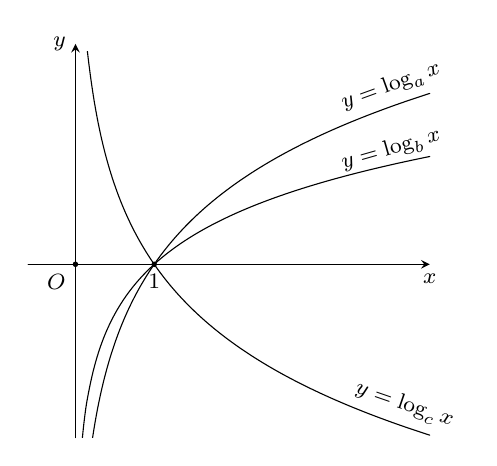
\begin{tikzpicture}[font=\footnotesize, line join=round, line cap=round, >=stealth, scale=1]
			\def\xmin{-0.6}
			\def\xmax{4.5}
			\def\ymin{-2.2}
			\def\ymax{2.8}
			\draw[->](\xmin,0)--(\xmax,0)node [below]{$x$};
			\draw[->](0,\ymin)--(0,\ymax)node [left] {$y$};
			\clip(\xmin,\ymin) rectangle (\xmax+0.5,\ymax-0.1);
			\fill (0,0) node[below left]{$O$} circle(1pt)
			(1,0) node[below]{$1$} circle(1pt);
			\draw[smooth,samples=100] plot[domain=0.1:\xmax](\x,{ln(\x)/ln(2)})node[shift={(170:0.5)}, rotate=20]{$y=\log_ax$};
			\draw[smooth,samples=100] plot[domain=0.04:\xmax](\x,{ln(\x)/ln(3)})node[shift={(170:0.5)}, rotate=16]{$y=\log_bx$};
			\draw[smooth,samples=100] plot[domain=0.1:\xmax](\x,{-ln(\x)/ln(2)})node[shift={(130:0.5)}, rotate=-19]{$y=\log_cx$};
		\end{tikzpicture}
	\end{center}
	\choiceTF
	{\True Trong các hàm số $y=\log_ax$, $y=\log_bx$, $y=\log_cx$ có đúng hai hàm số đồng biến trên tập xác định của nó}
	{$\log_cx>\log_c2\Rightarrow x<2$}
	{$\log(a+b+8c)<1+\log c$}
	{\True Đường thẳng $y=3$ cắt trục $Oy$, đồ thị các hàm số $y=\log_ax$, $y=\log_bx$ lần lượt tại $H$, $M$, $N$ sao cho $M$ là trung điểm của $HN$. Khi đó $2a^3=b^3$}
	\loigiai{
		\begin{itemchoice}
			\itemch
			Trong các hàm số $y=\log_ax$, $y=\log_bx$, $y=\log_cx$ có hai hàm số $y=\log_ax$ và $y=\log_bx$ đồng biến trên tập xác định của nó.
			\itemch 
			Hàm số $y=\log_cx$ là hàm nghịch biến nên $\log_cx>\log_c2\Leftrightarrow 0<x<2$.
			\itemch 
			Nếu $\log(a+b+8c)<1+\log c\Leftrightarrow\log(a+b+8c)<\log(10c)\Rightarrow a+b+8c<10c\Rightarrow a+b<2c$.\\
			Điều này không thể vì $a>1$, $b>1$ và $0<c<1$.
			\itemch 
			Đường thẳng $y=3$ cắt trục $Oy$, đồ thị các hàm số $y=\log_ax$, $y=\log_bx$ lần lượt tại $H(0;3)$, $M\left(a^3;3\right)$, $N\left(b^3;3\right)$.\\
			Ta có $M$ là trung điểm của $HN$ suy ra $0+b^3=2a^3$ hay $2a^3=b^3$.
		\end{itemchoice}
	}
\end{ex}
\Closesolutionfile{ans}


\ind{PHẦN III.} \inden{Trả lời ngắn.}\\
\setcounter{ex}{0}
\Opensolutionfile{ans}[ans/1D6-Bai4-KQ]

\begin{ex}[Trích đề thi HKIII - Sở Bắc Giang - Năm học 2023-2024]%[1D6H4-4]%[Dự án đề cương 3 Khối NH 24-25- Dot 1- Nguyễn Trần Anh Tuấn]
	Biết phương trình $2^{x^2-2x}=8$ có hai nghiệm phân biệt $x_1$ và $x_2$. Giá giá trị của biểu thức $S=x_1+x_2$ bằng bao nhiêu?
	
	\shortans[]{2}
	\loigiai
	{
		Ta có 
		\[
		2^{x^2-2x}=8 \Leftrightarrow x^2-2x=3 \Leftrightarrow x^2-2x-3=0 \Leftrightarrow \hoac{&x=-1\\ &x=3.}
		\]
		Vậy $S=x_1+x_2=2$.
	}
\end{ex}

\begin{ex}[Trích đề thi KSCL HKII - Sở GD Nam Định - Năm học 2024-2025]%[1D6H4-4]%[Dự án đề cương 3 Khối NH 24-25- Dot 1- Nguyễn Trần Anh Tuấn]
	Biết phương trình $3^{x^2+x+2} = \dfrac{1}{3^{2x-1}}$ có hai nghiệm phân biệt $x_1$, $x_2$. Giá trị biểu thức $T=x_1^2+x_2^2$ bằng bao nhiêu?
	\shortans[oly]{7}
	\loigiai{
		Ta có 
		\[3^{x^2+x+2}=3^{-(2x-1)}\Leftrightarrow x^2-x+2=-2x+1\Leftrightarrow x^2+3x+1=0.\]
		Khi đó $T= x_1^2+x_2^2=(x_1+x_2)^2-2x_1x_2=9-2=7$. 
	}
\end{ex}



\begin{ex}[Trích đề thi HKIII - THPT Nguyễn Khuyến, Bình Dương - Năm học 2024-2025]%[1D6H4-4]%[Dự án đề cương 3 Khối NH 24-25- Dot 1- Nguyễn Trần Anh Tuấn]
	Phương trình $\ln (x^2-3x+1)=\ln\left(x-2\right)$ có bao nhiêu nghiệm?
	
	\shortans[0]{1}
	\loigiai{
		Ta có $\ln (x^2-3x+1)=\ln\left(x-2\right)\Leftrightarrow \heva{&x-2>0\\&x^2-3x+1=x-2}\Leftrightarrow \heva{&x>2\\&\hoac{&x=3\\&x=1}}\Leftrightarrow x=3$.\\
		Vậy phương trình có $1$ nghiệm.
	}
\end{ex}



\begin{ex}%[1D6H4-5]%[Dự án đề cương 3 Khối NH 24-25- Dot 1- Nguyễn Trần Anh Tuấn]
	Tìm nghiệm nguyên nhỏ nhất của bất phương trình $\log_3\left(13-x^2\right)>2$.
	
	\shortans[]{-1}
	\loigiai{
		\begin{eqnarray*}
			\log_3\left(13-x^2\right)>2&\Leftrightarrow& \heva{&13-x^2>0\\&13-x^2>3^2}\\
			&\Leftrightarrow& \heva{&-\sqrt{13}<x<\sqrt{13}\\&-2<x<2}\\
			&\Leftrightarrow& -2<x<2.
		\end{eqnarray*}
		Mà $x\in\mathbb{Z}$ nên $x\in\{-1;0;1\}$. Vậy nghiệm nguyên nhỏ nhất của bất phương trình đã cho là $-1$.
	}
\end{ex}


\begin{ex}%[1D6V4-6]%[Dự án đề cương 3 Khối NH 24-25- Dot 1- Nguyễn Trần Anh Tuấn]
	Số lượng tế bào còn sống trong khoảng thời gian $t$ (phút) kể từ lúc tiến hành thí nghiệm được xác định bởi $f(t)=m\cdot \mathrm{e}^{nt}$ trong đó $m,n$ là các hằng số cho trước. Nếu bắt đầu thí nghiệm sinh học với $5\,000\,000$ tế bào thì $46\%$ các tế bào sẽ chết sau mỗi phút, hỏi thời gian tối thiểu để còn ít hơn $2\,000$ tế bào (làm tròn kết quả đến hàng phần chục)? 
	\shortans[]{12,7}
	\loigiai{
		Ta có 
		\begin{itemize}
			\item Sau một phút còn lại $0{,}54\cdot 5\cdot 10^6$ tế bào.
			\item Sau hai phút còn lại $0{,}54^2\cdot 5\cdot 10^6$ tế bào.
			\item Sau $t$ phút còn lại $0{,}54^t\cdot 5\cdot 10^6$ tế bào.
		\end{itemize}
		Theo đề bài ta có 
		\begin{align*} 0{,}54^t\cdot 5\cdot 10^6 <2\,000 \Rightarrow 0{,}54^t < \dfrac{1}{2\,500} \Rightarrow t> 12{,}7.
		\end{align*}
		Vậy thời gian tối thiểu để còn ít hơn $2\,000$ tế bào là $12{,}7$ phút.
	}
\end{ex}

\Closesolutionfile{ans}


\ind{PHẦN IV.} \inden{Tự luận.}\\
\setcounter{ex}{0}

\begin{ex}%[1D6H4-4]%[Dự án đề cương 3 Khối NH 24-25- Dot 1- Nguyễn Trần Anh Tuấn]
	Giải mỗi phương trình sau
	\begin{listEX}[2]
		\item $(0{,}3)^{x-3}=1$;
		\item $5^{3x-2}=25$;
		\item $9^{x-2}=243^{x+1}$;
		\item $\log_{\frac{1}{2}} (x+1)=-3$;
		\item $\log_5 (3x-5) =\log_5 (2x+1)$;
		\item $\log_{\frac{1}{7}}(x+9)=\log_{\frac{1}{7}} (2x-1)$.
	\end{listEX}
	\loigiai{
		Ta có
		\begin{enumerate}
			\item  $(0{,}3)^{x-3}=1 \Leftrightarrow x-3=\log_{0{,}3} 1\Leftrightarrow x-3=0 \Leftrightarrow x=3$.\\
			Vậy phương trình có nghiệm là $x=3$.
			\item  $5^{3x-2}=25 \Leftrightarrow 3x-2=\log_5 25 \Leftrightarrow 3x-2=2 \Leftrightarrow 3x=4 \Leftrightarrow x=\dfrac{4}{3}$.\\
			Vậy phương trình có nghiệm là $x=\dfrac{4}{3}$.
			\item  Ta có
			\begin{eqnarray*}
				9^{x-2}=243^{x+1} &\Leftrightarrow& 3^{2(x-2)} = 3^{5(x+1)}\\
				&\Leftrightarrow& 2(x-2)=5(x+1) \\
				&\Leftrightarrow& 2x-4=5x+5\\
				&\Leftrightarrow& -3x=9 \\
				&\Leftrightarrow& x=-3.
			\end{eqnarray*}
			Vậy phương trình có nghiệm là $x=-3$.
			\item $\log_{\frac{1}{2}} (x+1)=-3 \Leftrightarrow x+1=\left(\dfrac{1}{2}\right)^{-3} \Leftrightarrow x+1=8 \Leftrightarrow x=7$.\\
			Vậy phương trình có nghiệm là $x=7$.
			\item   $\log_5 (3x-5) =\log_5 (2x+1)$\\
			Điều kiện: $
			\heva{
				&3x-5>0\\
				&2x+1>0
			}\Leftrightarrow \heva{
				&x>\dfrac{5}{3}\\
				&x>-\dfrac{1}{2}
			} \Leftrightarrow x>\dfrac{5}{3}.
			$\\
			Phương trình đã cho $\log_5 (3x-5) =\log_5 (2x+1)$
			\[
			\Leftrightarrow 
			\heva{
				&x>\dfrac{5}{3}\\
				&3x-5=2x+1
			} \Leftrightarrow
			\heva{
				&x>\dfrac{5}{3}\\
				&x=6
			} \Leftrightarrow x=6.\]
			Vậy phương trình có nghiệm là $x=6$.
			\item  Phương trình $\log_{\frac{1}{7}}(x+9)=\log_{\frac{1}{7}} (2x-1)
			\Leftrightarrow 
			\heva{
				&x+9>0\\
				&x+9=2x-1
			} \Leftrightarrow
			\heva{
				&x>-9\\
				&x=10
			} \Leftrightarrow x=10.
			$\\
			Vậy phương trình có nghiệm là $x=10$.
		\end{enumerate}
	}
\end{ex}

\begin{ex}%[1D6H4-5]%[Dự án đề cương 3 Khối NH 24-25- Dot 1- Nguyễn Trần Anh Tuấn]
	Giải mỗi bất phương trình sau
	\begin{listEX}[2]
		\item $3^x>\dfrac{1}{243}$;
		\item $\left(\dfrac{2}{3}\right)^{3x-7}\leq \dfrac{3}{2}$;
		\item $4^{x+3}\geq 32^x$;
		\item $\log (x-1)<0$;
		\item $\log_{\frac{1}{2}}(2x-1)\geq \log_{\frac{1}{2}} (x+3)$;
		\item $\ln (x+3)\geq \ln (2x-8)$.
	\end{listEX}
	\loigiai{
		Ta có
		\begin{enumerate}
			\item  $3^x>\dfrac{1}{243} \Leftrightarrow x>\log_3 \dfrac{1}{243} \Leftrightarrow x>-5$.\\
			Vậy tập nghiệm của bất phương trình là $(-5;+\infty)$.
			\item  $\left(\dfrac{2}{3}\right)^{3x-7}\leq \dfrac{3}{2}
			\Leftrightarrow 3x-7 \geq \log_{\frac{2}{3}} \dfrac{3}{2}\Leftrightarrow 3x\geq 6 \Leftrightarrow x\geq  2$.\\
			Vậy tập nghiệm của bất phương trình là $[2;+\infty)$.
			\item  $4^{x+3}\geq 32^x \Leftrightarrow 2^{2(x+3} \geq 2^{5x} \Leftrightarrow 2(x+3)\geq 5x \Leftrightarrow -3x \geq -6 \Leftrightarrow x\leq 2$.\\
			Vậy tập nghiệm của bất phương trình là $(-\infty;2]$.
			\item   $\log (x-1)<0 \Leftrightarrow \heva{
				&x-1>0\\
				&x-1<10^0
			} \Leftrightarrow \heva{
				&x>1\\
				&x<2
			} \Leftrightarrow 1<x<2$.\\
			Vậy tập nghiệm của bất phương trình là $(1;2)$.
			\item  Bất phương trình $\log_{\frac{1}{2}}(2x-1)\geq \log_{\frac{1}{2}} (x+3)$
			\[
			\Leftrightarrow \heva{
				&2x-1>0\\
				& 2x-1 \leq x+3
			} \Leftrightarrow 
			\heva{
				&x>\dfrac{1}{2}\\
				&x\leq  4
			} \Leftrightarrow \dfrac{1}{2}<x\leq 4.
			\]
			Vậy tập nghiệm của bất phương trình là $\left(\dfrac{1}{2};4\right]$.
			\item  $\ln (x+3)\geq \ln (2x-8) \Leftrightarrow
			\heva{
				&2x-8>0\\
				&x+3\geq 2x-8
			}\Leftrightarrow
			\heva{
				&x>4\\
				&x\leq 11
			} \Leftrightarrow 4<x\leq 11
			$.\\
			Vậy tập nghiệm của bất phương trình là $\left(4;11\right]$.
		\end{enumerate}
	}
\end{ex}

\begin{ex}[Trích đề thi HKII - Sở Bắc Giang - Năm học 2024-2025]%[1D6H4-5]%[Dự án đề cương 3 Khối NH 24-25- Dot 1- Nguyễn Trần Anh Tuấn]
	Giải bất phương trình $\mathrm{e}^{x^2-2x-3} \geq 1$ .
	\loigiai{
		Ta có $ \mathrm{e}^{x^2-2x-3} \geq 1 \Leftrightarrow  x^2-2x-3\ge 0 \Leftrightarrow \hoac{&x \ge 1\\&x\le -3.}$\\
		Vậy tập nghiệm của bất phương trình là $\left(-\infty;-3\right] \cup [1;+\infty)$.
	}
\end{ex}


\begin{ex}%[1D6H4-4]%[Dự án đề cương 3 Khối NH 24-25- Dot 1- Nguyễn Trần Anh Tuấn]
	Giải phương trình $\log_{2}\bigl(3x-\sqrt{3} \bigr)+2\log _{\tfrac{1}{4}} \bigl(x+2\sqrt{3} \bigr)=0$.
	\loigiai{
		Điều kiện $x \ge \dfrac{\sqrt{3}}{3}$. Ta có
		\allowdisplaybreaks
		\begin{eqnarray*}
			&&\log_{2}\bigl(3x-\sqrt{3} \bigr)+2\log _{\tfrac{1}{4}} \bigl(x+2\sqrt{3} \bigr)=0\\
			&\Leftrightarrow& \log_{2}\bigl(3x-\sqrt{3} \bigr)-\log _{2}\bigl(x+2\sqrt{3} \bigr)=0		\\
			&\Leftrightarrow& \log_{2}\bigl(3x-\sqrt{3} \bigr)=\log _{2}\bigl(x+2\sqrt{3} \bigr)\\
			&\Leftrightarrow& 3x-\sqrt{3}=x+2\sqrt{3}\\
			&\Leftrightarrow & x= \dfrac{3\sqrt{3}}{2}.
		\end{eqnarray*}
		Thử lại ta thấy $x= \dfrac{3\sqrt{3}}{2}$ là nghiệm của phương trình đã cho.\\
	}
\end{ex}

\begin{ex}[Trích đề thi HKII - THPT Nhân Chính Hà Nội - Năm học 2023-2024]%[1D6V4-5]%[Dự án đề cương 3 Khối NH 24-25- Dot 1- Nguyễn Trần Anh Tuấn]
	Có bao nhiêu số nguyên dương là nghiệm của bất phương trình $\log_2\dfrac{1}{x^2-x}+\log_2x+1\ge 0$?
	\loigiai{
		Điều kiện: $\heva{&x^2-x>0\\&x>0}\Leftrightarrow x>1$.\\
		Bất phương trình tương đương với
		\begin{align*}
			&\,\log_2\dfrac{1}{x^2-x}+\log_2x+1\ge 0\\ \Leftrightarrow &\,\log_2x+\log_22\ge \log_2\left(x^2-x\right)\\
			\Leftrightarrow &\,\log_2(2x)\ge \log_2\left(x^2-x\right)\\
			\Leftrightarrow &\, 2x\geq x^2-x\\
			\Leftrightarrow &\, 0\leq x\leq 3.
		\end{align*}
		Vì $x>1$ nên $1<x\le3$.\\
		Vậy có $2$ số nguyên dương thỏa mãn bất phương trình.
	}
\end{ex}

\begin{ex}%[1D6V4-6]%[Dự án đề cương 3 Khối NH 24-25- Dot 1- Nguyễn Trần Anh Tuấn]
	Sử dụng công thức tính mức cường độ âm $L$ ở ví dụ $14$, hãy tính mức cường độ âm mà tai người có thể nghe được, biết rằng tai nguời có thể nghe được âm với cường độ âm từ $10^{-12}$ W/m$^2$ đến $10$ W/m$^2$.
	\loigiai{
		Ta có công thức mức cường độ âm $L=10\log \dfrac{I}{10^{-12}}$, trong đó $I$ (đơn vị: W/m$^2$) là cường độ âm.\\
		Mức cường độ âm mà tai người có thể nghe được là
		\[
		10\log \dfrac{10^{-12}}{10^{-12}}<L<10\log \dfrac{10}{10^{-12}}
		\Leftrightarrow 0<L<130.
		\]
		Vậy mức cường độ âm mà tai người nghe được từ $0$ đến $130$ dB.
	}
\end{ex}


\begin{ex}[Trích đề thi KSCL - Sở Lạng Sơn - Năm học 2023-2024]%[1D6V4-6]%[Dự án đề cương 3 Khối NH 24-25- Dot 1- Nguyễn Trần Anh Tuấn]
	Trong quá trình nuôi cấy một loại vi khuẩn, nếu gọi $N(t)$ là số lượng vi khuẩn sau $t$ giờ thì ta có $N(t) = N_0 \cdot \mathrm{e}^{r t}$, trong đó $N_0$ là số lượng vi khuẩn ban đầu và $r$ là tỉ lệ tăng trưởng vi khuẩn mỗi giờ. Biết rằng ban đầu có $1\,000$ con vi khuẩn và sau $2$ giờ số vi khuẩn là $3\,000$ con. Hỏi sau ít nhất bao nhiêu giờ thì số lượng vi khuẩn không ít hơn $9\,000$ con?
	
	\loigiai{
		Sau $2$ giờ số vi khuẩn là $3\,000$ con nên ta có
		\begin{eqnarray*}
			3\,000=1\,000 \cdot \mathrm{e}^{r\cdot 2}
			\Leftrightarrow \mathrm{e}^r = 3^{\tfrac{1}{2}}.
		\end{eqnarray*}
		Khi đó $N(t) = N_0 \cdot 3^{\tfrac{t}{2}}$.\\
		Ta có 
		\begin{eqnarray*}
			N(t)\ge 9\,000 \Leftrightarrow 1\,000\cdot 3^{\tfrac{t}{2}}\ge 9\,000
			\Leftrightarrow 3^{\tfrac{t}{2}} \ge 9
			\Leftrightarrow \dfrac{t}{2} \ge 2
			\Leftrightarrow t \ge 4.
		\end{eqnarray*}
		Vậy sau ít nhất $4$ giờ thì số lượng vi khuẩn không ít hơn $9\,000$ con.
	}
\end{ex}

\begin{ex}[Trích đề thi HKII - THPT Đông Anh, Hà Nội - Năm học 2023-2024]%[1D6H4-6]%[Dự án đề cương 3 Khối NH 24-25- Dot 1- Nguyễn Trần Anh Tuấn]
	Sau tết Nguyên Đán Giáp Thìn $2024$, tổng số tiền bạn Bình An được mừng tuổi là $4$ triệu đồng. Bạn quyết định để dành tiền đó cho một số tiêu dùng cần thiết khi trở thành tân sinh viên đại học sau $18$ tháng nữa. Bạn đã lựa chọn gửi tiết kiệm trong $18$ tháng theo kì hạn $3$ tháng, lãi suất $1{,}5\%$ trên một kì hạn với hình thức lãi kép, giả sử lãi suất không thay đổi và bạn Bình An không gửi thêm cũng như rút ra trong suốt $18$ tháng. Sau $18$ tháng, bạn Bình An nhận được số tiền cả lãi và gốc là bao nhiêu? (tính theo đơn vị triệu đồng, làm tròn tới hàng phần trăm)
	
	\loigiai{
		Áp dụng công thức lãi kép ta có số tiền bạn Bình An nhận được sau $18$ tháng (sau $6$ kì hạn) là
		\[T=A(1+r)^n=4(1+0{,}015)^6\approx 4{,}37 \text{ (triệu đồng)}.\]
	}
\end{ex}


\begin{ex}[Trích đề thi HKII - THPT Cẩm Bá Thước, Thanh Hóa - Năm học 2023-2024]%[1D6V5-5]%[Dự án đề cương 3 Khối NH 24-25- Dot 1- Nguyễn Trần Anh Tuấn]
	Sự tăng trưởng của một loại vi khuẩn tuân theo công thức $S=A \cdot {\mathrm{e}^{r \cdot t}}$, trong đó $A$ là số lượng vi khuẩn ban đầu, $r$ là tỉ lệ tăng trưởng $\left( r>0 \right)$, $t$ là thời gian tăng trưởng. Biết số lượng vi khuẩn ban đầu là $50$ con và sau $5$ giờ có được $250$ con. Hỏi sau ít nhất bao nhiêu giờ thì số vi khuẩn có được là trên $2$ triệu con (lấy số giờ là số nguyên)?
	\loigiai{
		Sự tăng trưởng của một loại vi khuẩn tuân theo công thức $S=A\cdot {\mathrm{e}^{r\cdot t}}$, trong đó $A$ là số lượng vi khuẩn ban đầu, $r$ là tỉ lệ tăng trưởng $\left( r>0 \right)$, $t$ là thời gian tăng trưởng.\\
		Số lượng vi khuẩn ban đầu là $50$ con và sau $5$ giờ là $250$ con, tức là $250=50\cdot {\mathrm{e}^{r\cdot 5}}\Leftrightarrow r=\dfrac{1}{5}\ln 5$.\\
		Số vi khuẩn có được là trên $2$ triệu con, nên ta có
		\[50\cdot {\mathrm{e}^{\left( \tfrac{1}{5}\ln 5 \right)\cdot t}}>2\,000\,000\Leftrightarrow {\mathrm{e}^{\left( \tfrac{1}{5}\ln 5 \right)\cdot t}}>40\, 000\Leftrightarrow t>\dfrac{5\ln 40\, 000}{\ln 5}\Leftrightarrow t>32{,}92.\]
		Vậy sau ít nhất $33$ giờ thì số vi khuẩn có được là trên $2$ triệu con.}
\end{ex}



\begin{ex}[Trích đề thi giữa HKII - Sở Hà Nội - Năm học 2023-2024]%[1D6H4-4]%[Dự án đề cương 3 Khối NH 24-25- Dot 1- Nguyễn Trần Anh Tuấn]
	Cho các hàm số $y=3^{3x+1}$ và $y=9^x$ có đồ thị lần lượt là $(C_1)$ và $(C_2)$. Gọi $A$ là giao điểm của $(C_1)$ và $(C_2)$. Gọi $B$, $C$ lần lượt là giao điểm của trục $Oy$ với $(C_1)$ và $(C_2)$. Tính Diện tích của tam giác $ABC$.
	\loigiai{
		Phương trình hoành độ giao điểm của $(C_1)$ và $(C_2)$ là 
		\begin{align*}
			3^{3x+1}=9^x\Leftrightarrow 3x+1=2x
			\Leftrightarrow x=-1.
		\end{align*}
		Suy ra $A\left(-1;\dfrac{1}{9}\right)$.\\
		Giao điểm của $(C_1)$ và $Oy$ là $B(0;3)$, giao điểm của $(C_2)$ và $Oy$ là $C(0;1)$.\\
		Suy ra $BC=|y_B-y_C|=|3-1|=2$.\\
		Ta có $\mathrm{d}(A,BC)=\mathrm{d}(A,Oy)=|x_A|=1$.\\
		Vậy diện tích tam giác $ABC$ là 
		\begin{align*}
			S_{\triangle ABC}=\dfrac{1}{2}\cdot BC\cdot \mathrm{d}(A,BC)=\dfrac{1}{2}\cdot 2\cdot 1=1.
		\end{align*}
	}
\end{ex}